\documentclass[10pt]{article}
\usepackage[utf8]{inputenc}
\usepackage{url}
\usepackage{graphicx}
\usepackage[table]{xcolor}
\usepackage{blindtext}
\usepackage{enumitem}
\usepackage{booktabs}

\title{First document}
\author{Group 3}
\date{October 2018}
\begin{document}

\section{Sprint Planning}

\subsection{Overview}

In the beginning of every iteration features are chosen for that iteration and are broken down into specific tasks that are then allocated to the team members. These tasks are also called the sprint backlog. Goals set for each sprint are used as a guideline for features that are selected for that sprint. Task take 4 hours to 4 days depending on their level of difficulty and level of knowledge of the member that the task is assigned to.

\subsection{Roles}

Team leader - Mpinane Mohale
Team member - Thulisile shipyana
Team member -  Sbusiso Mkhombe
Team member - Lucky Mahlangu

\subsection{Product Backlog}

\begin{description}[font=$\bullet$~\normalfont\scshape\color{red!50!black}]

\item [] As a student I want to be able to register on the system so that I can have access to the services provided by the systemion.
\item [] As a student I want to be able to add course that I have completed and also the marks obtained on them so that I can get a recommendation(s) of the courses I can take for my post graduate studies.
\item [] As a student I want to get the predicted marks on the recommended courses so that I can decide on which courses to enroll for.
\end{description}

\begin{center}
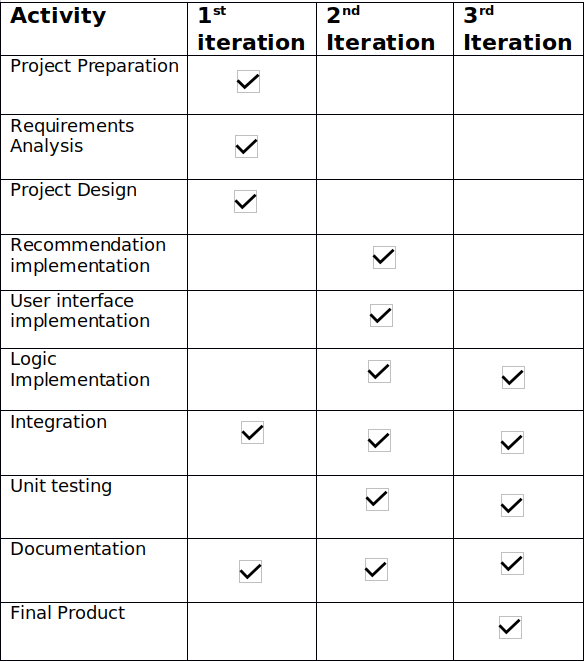
\includegraphics[width=.9\textwidth]{activity.png}
\end{center}
\caption{\underline{Iteration Table}}
The table above shows a simplified activity plan that was carried out. 

\subsection{First Iteration}

\subsubsection{Objectives}

This iteration aims to gather the requirements of the system and to design the system architecture together with the system interface also determining the overall feasibility of the project

\subsubsection{Tasks}

Documentation (all members worked on the documentation)

\subsubsection{Sprint Retrospective}

What worked: Goals of the sprint where achieved and everything was done on time, team collaboration
What was challenging/ didn’t work:  having to learn the Django design patterns with limited time, generating the data for training the classifier 
How was it resolved: attacked the problem bit by bit, each member had to take Django tutorials in order to familiarize themselves with it.

\subsection{Second Iteration}

\subsubsection{Objectives}

In this iteration, we will focus on the implementation of three elements, namely the user interface, the login and the registration page with the functionality, and the course recommendation. We will also conduct unit test on the implemented tasks.

\subsubsection{Task}

“As a student I want to be able to register on the system so that I can have access to the services provided by the system”.

“As a student I want to be able to add courses that I have completed together with the marks achieved so that I can get recommendations of the elective courses that I can take for my post graduate degree”.

\begin{description}[font=$\bullet$~\normalfont\scshape\color{red!50!black}]

\item [] Implementation of the login and registration – Mpinane, Sbusiso.
\item [] Add courses page, create the UI - Thulisile.
\item [] Conduct unit testing - Sbusiso.
\item [] Add the course in the database - Thulisile.
\item [] Add the recommendation page, create UI - Mpinane.
\item [] Generate data - Lucky Mahlangu.
\item [] Create the recommendation function using machine learning techniques – Lucky Mahlangu.
\end{description}

\subsubsection{Acceptance Criteria}

\begin{description}[font=$\bullet$~\normalfont\scshape\color{red!50!black}]

\item [] User should be able to register. 
\item [] User should be to retrieve the saved courses.
\item [] User should be able to delete and edit the courses.
\item [] User should be able to get recommendations based on the added coursed and their marks.

\end{description}

\subsubsection{Sprint Retrospective}

What worked: where a member struggle with a particular task, other members were able to assist or refer them where they can find help, team collaboration.

What was challenging/ didn’t work:

\begin{description}[font=$\bullet$~\normalfont\scshape\color{red!50!black}]

\item [] Other things took time to implement.
\item [] Some tasks took longer than anticipated.
\item [] Some meetings were not effective. 
\item [] Deciding on which features to implement and getting user stories   right the first time.
\item [] Members arriving late to the meetings.

\end{description}

How was it resolved: We broke the tasks further into smaller tasks which also helped in them being completed in the estimated time. Meetings time was reduced to an hour, the team reached a consensus.
What could have been done: We could have updated the documentation in line with the code changes. 

\subsection{Third Iteration}

\subsubsection{Objectives}

In this iteration, we will continue to add functionality to the web pages created in the previous iteration and also to extend the course recommendation to include the marks predictions. Unit test was also conducted for the code implemented in this iteration.

\subsubsection{Tasks}

“As a student I want to get the predicted marks on the recommended courses so that I can decide on which courses to enroll for”.

\begin{description}[font=$\bullet$~\normalfont\scshape\color{red!50!black}]

\item [] Implement the marks prediction - Lucky.
\item [] Unit testing – Sbusiso.
\item [] Logic implementation – Mpinane, Thulisile.

\end{description}

\subsubsection{Acceptance Criteria}

\begin{description}[font=$\bullet$~\normalfont\scshape\color{red!50!black}]

\item [] User should be able to get the predicted mark of the recommended courses.
\item [] All the web pages should have the expected functionality, i.e.  the user should be directed to the page they have requested. 
\item [] User should be able to update their account.

\end{description}

What worked: team collaboration, incorporating lessons learned in the previous iterations in to this one.

What was challenging/ didn’t work: some members were not doing small commits.

How was it resolved: we introduced a rule that members have to commit no matter how small the commits.

What could have been done: We could have used a planning tools to track our progress, task time estimation. We could have done more interesting retrospective formats.

\subsubsection{Definitions}

\textbf{Product Backlog} - these are the features to be implemented for the whole project, they are in a form of a user story, i.e. the sentence inside the " ".

\textbf{User story} – is a tool used to capture a description of a feature from an end-user perspective, format: As a <user type>, I want <goal> so that < reason>.

\textbf{Sprint backlog} - is a subset of the product backlog, that is chosen by the team and broken down into manageable tasks and prioritized and completed in the sprint.

\textbf{Acceptance criteria} - is when a task item is complete and working as expected.

\end{document}